\section{Experiment}
In this section, we experiment on task-specific language model compression. We introduce the datasets for evaluation and baseline methods for comparison. Then we show the 
quantitative results followed by ablation study and analysis.
\subsection{Datasets}
We experiment on five diverse natural language understanding tasks: sentiment classification, paraphrase detection, natural language inference, 
linguistic acceptability, and semantic textual similarity.
We use the following datasets:
SST-2~\cite{sst2} is a movie review dataset with positive/negative annotations for binary sentiment classification. Accuracy is used as the test metric; MRPC~\cite{mrpc} contains pairs of sentences with binary labels indicating the semantic equivalence relationship. F1 score is used as the test metric;
 RTE~\cite{rte} is a textual entailment challenge with binary annotations. Accuracy is used as the test metric;
 CoLA~\cite{cola} contains sentences labeled as grammatical or ungrammatical from linguistic literature. Matthew's correlation is used as the test metric;
 STS-B~\cite{stsb} contains pair of sentences labeled with 1-5 scores as their semantic similarity. Spearman correlation is used as the test metric.
\subsection{Baselines}
We compare LCD against baselines with and without KD. We exclude TinyBERT~\cite{tinybert} because it involves an extra pre-training stage beyond task-specific data.

\textbf{KD-based methods:}
% \begin{itemize}
%     \item RKD~\cite{kd} applies KD objective only on the final output of teacher and student networks.
%     \item PKD~\cite{pkd} proposed patient-based knowledge distillation that minimizes the mean-square-error between hidden states of each student layer and its one-to-one mapped teacher layer.
%     \item CKD~\cite{ckd} allows one-to-many mapping and minimizes the mean-square-error between the hidden state of each student layer and a convex combination of hidden states from its mapped teacher layers.
%     \item ALP-KD~\cite{alpkd} further enhances CKD by allowing one-to-all mapping and minimizing the mean-square-error between the hidden state of each student layer and a convex combination of hidden states from all teacher layers.
% \end{itemize}
\textbf{RKD}~\cite{kd} applies KD objective only on the final output of teacher and student networks. \textbf{PKD}~\cite{pkd} proposed patient-based knowledge distillation that minimizes the mean-square-error between hidden states of each student layer and its one-to-one mapped teacher layer.
 \textbf{CKD}~\cite{ckd} allows one-to-many mapping and minimizes the mean-square-error between the hidden state of each student layer and a convex combination of hidden states from its mapped teacher layers.
\textbf{ALP-KD}~\cite{alpkd} further enhances CKD by allowing one-to-all mapping and minimizing the mean-square-error between the hidden state of each student layer and a convex combination of hidden states from all teacher layers.

\textbf{KD-free methods:}
% \begin{itemize}
%     \item Fine-tuning, which truncates the large pre-trained language model into the size of the compressed model and directly fine-tunes it using task-specific objective.
%     \item LayerDrop~\cite{layerdrop} applies structured dropout on layers randomly during training to make models robust to missing layers.
%     \item BERT-of-Theseus~\cite{theseus} is based on module replacement. It can be seen as a special case of LCD that only has one branch and trains without demonstration.
% \end{itemize}
\textbf{Fine-tuning}, which truncates the large pre-trained language model into the size of the compressed model and directly fine-tunes it using task-specific objective.
 \textbf{LayerDrop}~\cite{layerdrop} applies dropout on layers randomly during training to make models robust to missing layers.
\textbf{BERT-of-Theseus}~\cite{theseus} is based on module replacement. It can be seen as a special case of LCD that only has one branch and trains without demonstration.

\subsection{Implementation Details}
We use the publically available 12-layer BERT-base\footnote{\url{https://github.com/QData/TextAttack}} model fine-tuned for each task as the teacher network for all KD-based baselines, BERT-of-Theseus, and our LCD. For the 
compression target, we consider a shallower counterpart of BERT with 4/6 layers and initialize it using the corresponding layers from the teacher following \cite{theseus}. The compressed model offers about 2.82x/1.94x inference speed up and 52\%/38\% size reduction. 

\begin{table*}[t]
    \centering
    \scriptsize
    \begin{tabular}{l|lllll|l}
    \toprule
    Models            & SST-2 & MRPC & RTE  & CoLA & STS-B & Avg.  \\
    \midrule
    BERT-base$_{12}$         & 92.4  & 88.9 & 72.5 & 53.0 & 87.7  & 78.9 \\
    \midrule
    \cellcolor[HTML]{EFEFEF}\textbf{\textit{KD-based}}  & & & & & & \\
    RKD$_4$               & 89.0  & 84.8 & 62.8 & 28.2 & 86.2  & 70.2 \\
    PKD$_4$               & 89.2  & 84.8 & 62.4 & 27.6 & 86.2  & 70.0 \\
    CKD$_4$              & 89.4  & 85.5 & 62.2 & 29.7 & 86.3  & 70.6 \\
    ALP-KD$_4$            & 89.0  & 85.2 & 62.4 & 26.9 & 86.4  & 70.1 \\
    \midrule
    \cellcolor[HTML]{EFEFEF}\textbf{\textit{KD-free}}  & & & & & & \\
    Fine-tuning$_4$       & 89.0  & 84.9 & 62.2 & 27.2 & 86.1  & 69.9 \\
    LayerDrop$_4$         & 87.9  & 82.8 & 59.2 & 26.0 & 82.8  & 66.9 \\
    BERT-of-Theseus$_4$   & 89.2  & 86.6 & 63.2 & 33.5 & 86.5  & 71.8 \\
    \midrule
    \cellcolor[HTML]{EFEFEF}\textbf{\textit{Ours}}  & & & & & & \\
    LC$_4$                & 89.5  & 86.7 & 63.9 & 33.6 & 86.6  & 72.1 \\
    LCD$_4$               & \underline{90.3$^*$}  & \underline{88.9$^*$} & \underline{65.1$^*$} & \underline{36.0$^*$} & \underline{87.4$^*$}  & \underline{73.5$^*$} \\
    LCD$_4^{Aug}$       & \textbf{90.9$^*$}  & \textbf{89.3$^*$} & \textbf{65.7$^*$} & \textbf{37.7$^*$} & \textbf{87.7$^*$}  & \textbf{74.3$^*$} \\
    \bottomrule
    \end{tabular}
  \quad
  \quad
    \centering
    \scriptsize
    \begin{tabular}{l|lllll|l}
    \toprule
    Models            & SST-2 & MRPC & RTE  & CoLA & STS-B & Avg.  \\
    \midrule
    BERT-base$_{12}$         & 92.4  & 88.9 & 72.5 & 53.0 & 87.7  & 78.9 \\
    \midrule
    \cellcolor[HTML]{EFEFEF}\textbf{\textit{KD-based}}  & & & & & & \\
    RKD$_6$               &91.2   &88.2  &63.4  &43.2  &87.8   &74.8  \\
    PKD$_6$               &91.5   &88.0  &63.7  &43.6  &87.8   &74.9  \\
    CKD$_6$               &91.4   &88.3  &63.8  &44.6  &88.0   &75.2  \\
    ALP-KD$_6$            &91.5   &87.8  &63.9  &43.8  &87.8   &75.0  \\
    \midrule
    \cellcolor[HTML]{EFEFEF}\textbf{\textit{KD-free}}  & & & & & & \\
    Fine-tuning$_6$       &91.2   &87.6  &63.0  &43.8  &87.7   &74.7  \\
    LayerDrop$_6$         &90.6   &88.1  &63.2  &41.8  &85.1   &73.8  \\
    BERT-of-Theseus$_6$   &91.6   &90.4  &64.9  &45.0  &88.0   &76.0  \\
    \midrule
    \cellcolor[HTML]{EFEFEF}\textbf{\textit{Ours}}  & & & & & & \\
    LC$_6$                &91.6   &90.4  &65.2  &45.5  &88.1   &76.2  \\
    LCD$_6$               & \underline{91.8}  & \underline{90.8} & \underline{65.5} & \textbf{47.3$^*$} & \underline{88.3$^*$}  & \underline{76.8} \\
    LCD$_6^{Aug}$       & \textbf{92.0}  & \textbf{91.4$^*$} & \textbf{66.6$^*$} & \underline{47.2$^*$} & \textbf{88.4$^*$}  & \textbf{77.1$^*$} \\
    \bottomrule
    \end{tabular}
    \caption{Results of 4~(left) and 6~(right) layer student network, averaged over five runs. Subscript indicates the number of layers. LC refers to our framework without demonstration stage, LCD is the complete version with both stages. LCD$^{Aug}$ refers to LCD with data augmentation. 
    Best results are \textbf{bolded} and the second best are \underline{underlined}. $^*$ indicates statistical significance~($p<$0.05) measured by Student's T-Test.}
    \label{table:main}
  \end{table*}

We do not perform extensive hyper-parameter tuning due to the computation budget. We fix the batch size as 32 and set the max sequence length as 128 for all evaluated tasks. The training epochs are set to 17 for RTE, 5 for SST-2, and 15 for other tasks. AdamW~\cite{adamw} is used as the optimizer with a learning rate of 2e-5. The initial Bernoulli probability $p_{init}$ is fixed as 0.3 and $p$ will be reset to $p_{init}$ at the begining of each stage. The 
step size $k$ is set to 0.0006. For each task, we train with five random seeds from $\{12,42,100,128,256\}$ and report the average results. For data augmentation, we utilize a pre-trained paraphrasing model\footnote{\url{https://huggingface.co/eugenesiow/bart-paraphrase}}\cite{bart} to generate one paraphrased input for each task in the demonstration stage.


\subsection{Main Results}

We report the experimental results of both 4 and 6 layer compression targets in \tabref{table:main}. The results of all compared methods are reproduced by us under the same experimental environment based on their 
official implementations. For LayerDrop, we use the \textit{Every-Other} strategy recommended in the original paper for choosing student layers.

The 12-layer teacher network obtains the best performance across all tasks due to better generalization ability brought by over-parametrization. 
Surprisingly, LayerDrop performs worse than Fine-tuning, which is likely due to 
the lack of teacher supervision and noisy gradient given by layers that are not used in testing. Compared to Fine-tuning, all KD-based methods are able to deliver better 
performance. However, the improvements are somewhat marginal, e.g., at most 0.7 points by CKD. BERT-of-Theseus turns out to be the strongest baseline, showing that 
learning through interaction can more effectively transfer knowledge from teacher to student. Our 4/6-layer LCD retains 93.2\%/97.3\% of the averaged teacher performance, outperforming both KD-based and KD-free methods. 
Even without the demonstration stage, learning from collaboration alone based on our proposed two-branch container already performs better than all compared baselines. As mentioned before, LCD can easily incorporate 
any form of data augmentation without the need for label. With simple augmentation via paraphrasing, LCD$_{Aug}$ further attains 0.8/0.3 average improvement compared with LCD under 4/6 layer setting. We leave the exploration of other more sophisticated data augmentations for future work.

The advantage of LCD can be explained from three aspects. First, compared with KD-free methods that make no use of explicit supervision from the complete teacher network, LCD can exploit both implicit and explicit learning signals from the teacher. Second, though KD-based methods explicitly design 
distillation objectives for knowledge transfer, these objectives are jointly optimized with the task-specific objective, which requires careful tuning of relative weight and may suffer from conflictive gradients. LCD addresses this issue by separating these two types of 
objectives into two learning stages. Last, the underlying two-branch container allows deep interaction between student and teacher at the gradient level, improving the learning efficacy at both stages.


\subsection{Ablation Study}
\label{sec:ablation}
In this subsection, we demonstrate the impact of several technical designs of LCD by ablation study.

\subsubsection{Dynamic v.s. Static Probability}
\begin{table}[h!]
    \centering
    \scriptsize
    \begin{tabular}{l|ccccc|c}
    \toprule
    Models            & SST-2 & MRPC & RTE  & CoLA & STS-B & Avg.  \\
    \midrule
    \cellcolor[HTML]{EFEFEF}\textbf{\textit{Dynamic}}  & & & & & & \\
    LC$_4$                &89.5   &86.7  &63.9  &33.6  &86.6   &72.1  \\
    \midrule
    \cellcolor[HTML]{EFEFEF}\textbf{\textit{Static}}  & & & & & & \\
    LC$_4~$($p$=0.3)       &89.3   &86.4  &64.2  &32.4  &86.1   &71.7  \\
    LC$_4~$($p$=0.5)       &89.3  &86.9  &62.5  &32.1  &85.9  &71.3 \\
    LC$_4~$($p$=0.7)       &89.5  &86.4  &64.0  &32.6  &86.2  &71.7 \\
    \bottomrule
    \end{tabular}
    \caption{Ablation study on the probability scheduler.}
    \label{table:scheduler}
\end{table}
To study the impact of probability scheduler, we compare the results of LC$_4$ with a dynamic scheduler and with a 
static scheduler. The dynamic scheduler linearly increases $p$ from 0.3 to 1 while the static scheduler keeps a constant $p$ from $\{0.3, 0.5, 0.7\}$ throughout training. 


The results from \tabref{table:scheduler} shows that setting $p$ to constant gives a worse overall performance. The reason is that a constant $p$ makes the
framework almost never train all student layers together, whereas a dynamic scheduler 
will assign all student layers to the same branch late during training.

\subsubsection{Weighting Strategy}

\begin{table}[h!]
    \centering
    \scriptsize
    \begin{tabular}{l|ccccc|c}
    \toprule
    Models            & SST-2 & MRPC & RTE  & CoLA & STS-B & Avg.  \\
    \midrule
    LC$_4~$(\textit{pos})       &89.5   &86.7  &63.9  &33.6  &86.6   &72.1  \\
    LC$_4~$(\textit{neg})       &84.7  &86.8  &63.0  &26.9  &85.6   &69.4  \\
    \bottomrule
    \end{tabular}
    \caption{Ablation study on weighting strategy.}
    \label{table:weighting}
\end{table}

To study the impact of weighting strategy, we compare the results using two different strategies that weights positively or negatively with regard to
the number of student layers in each branch. 


The results are shown in \tabref{table:weighting}. Training with negative weighting strategy causes significant performance drops on almost all tasks. 
The reason is that, with negative weighting, the branch with the majority of student layers receives a diminishing learning signal while the other branch gets aggressively updated. This 
highlights the importance of letting each student layer trained with roughly the same scale of loss.

\subsubsection{Two-branch v.s. One-branch}
\begin{table}[h!]
    \centering
    \scriptsize
    \begin{tabular}{l|ccccc|c}
    \toprule
    Models            & SST-2 & MRPC & RTE  & CoLA & STS-B & Avg.  \\
    \midrule
    LCD$_4~$       &90.3   &88.9  &65.0  &36.0  &87.4   &73.5  \\
    LCD$_4~$(\textit{one-branch})       &90.2  &88.3  &65.0  &35.8  &86.3   &73.1  \\
    \bottomrule
    \end{tabular}
    \caption{Ablation study on branch design.}
    \label{table:archidemo}
\end{table}
To study the impact of our two-branch container design, we compare the results of LCD$_4$ againts a variant that keeps all student layers in one branch. They are both initialized from parameters after collaboration stage and are trained using the same 
distillation objective as in Eq 12.

\tabref{table:archidemo} shows that the two-branch LCD$_4$ consistently outperforms its one-branch variant on almost all tasks, demonstrating the advantage of fine-grained layer-wise teacher-student interaction for 
knowledge transfer.


\subsection{Analysis}
In this section, we analyze the compressed student network at both layer and model level on the development set of MRPC.
\subsubsection{Layer-level}
To examine the extent to which a student layer mimics its corresponding teacher layers, we 
conduct experiments on BERT-of-Theseus$_4$, LC$_4$ and LCD$_4$ by iteratively using one of their student layers to replace its corresponding 3 layers in the teacher network. We then observe how the replaced teacher performs and its representation similarity with the original teacher measured by Central Kernal Alignment~(CKA)\cite{cka}.


\begin{figure}[htb]
\centering
    % \scalebox{0.129}{
\includegraphics{./figures/layer_addtheseus.png}}
    \scalebox{0.225}{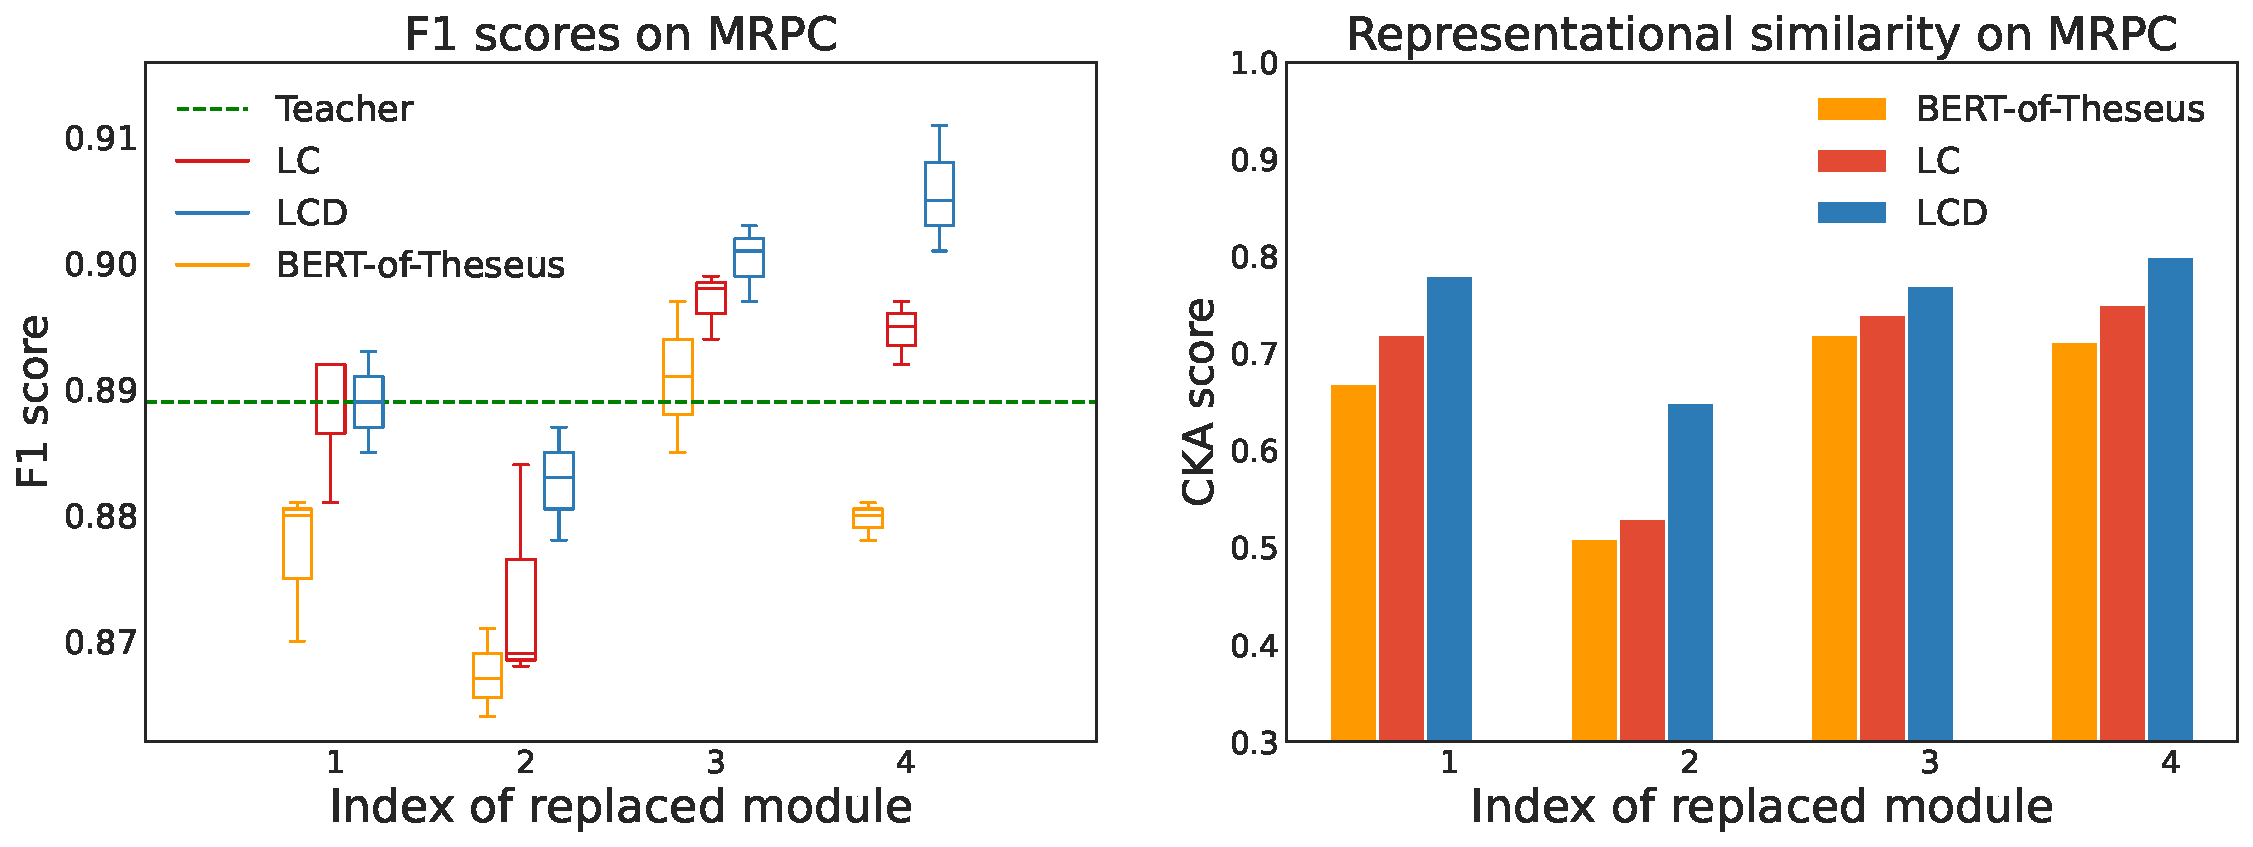
\includegraphics{./figures/cka_mrpc_addtheseus.pdf}}
    \caption{F1 scores and CKA similarity w.r.t. teacher network.}
    \label{fig:analysis_1}
\end{figure}

\figref{fig:analysis_1} shows that the replacement in earlier layers causes minor performance drop while the replacement in higher layers even improves the task performance over original teacher. This is because the gradient intensity exhibits gradual degradation when back-propagated from higher layers to lower layers, rendering the knowledge stored in lower layers more difficult to compress. 
Student layers trained by LC$_4$ better simulate its corresponding teacher layers than BERT-of-Theseus$_4$, verifying the advantage of our two-branch design over single-branch one. Replacement by LCD$_4$ consistently obtains a higher F1 score as well as a higher degree of alignment with the teacher's representation than LC$_4$. 
It suggests that learning from explicit demonstration improves the quality of knowledge transfer.

\subsubsection{Model-level}
\begin{figure}[htb]
\centering
    \scalebox{0.227}{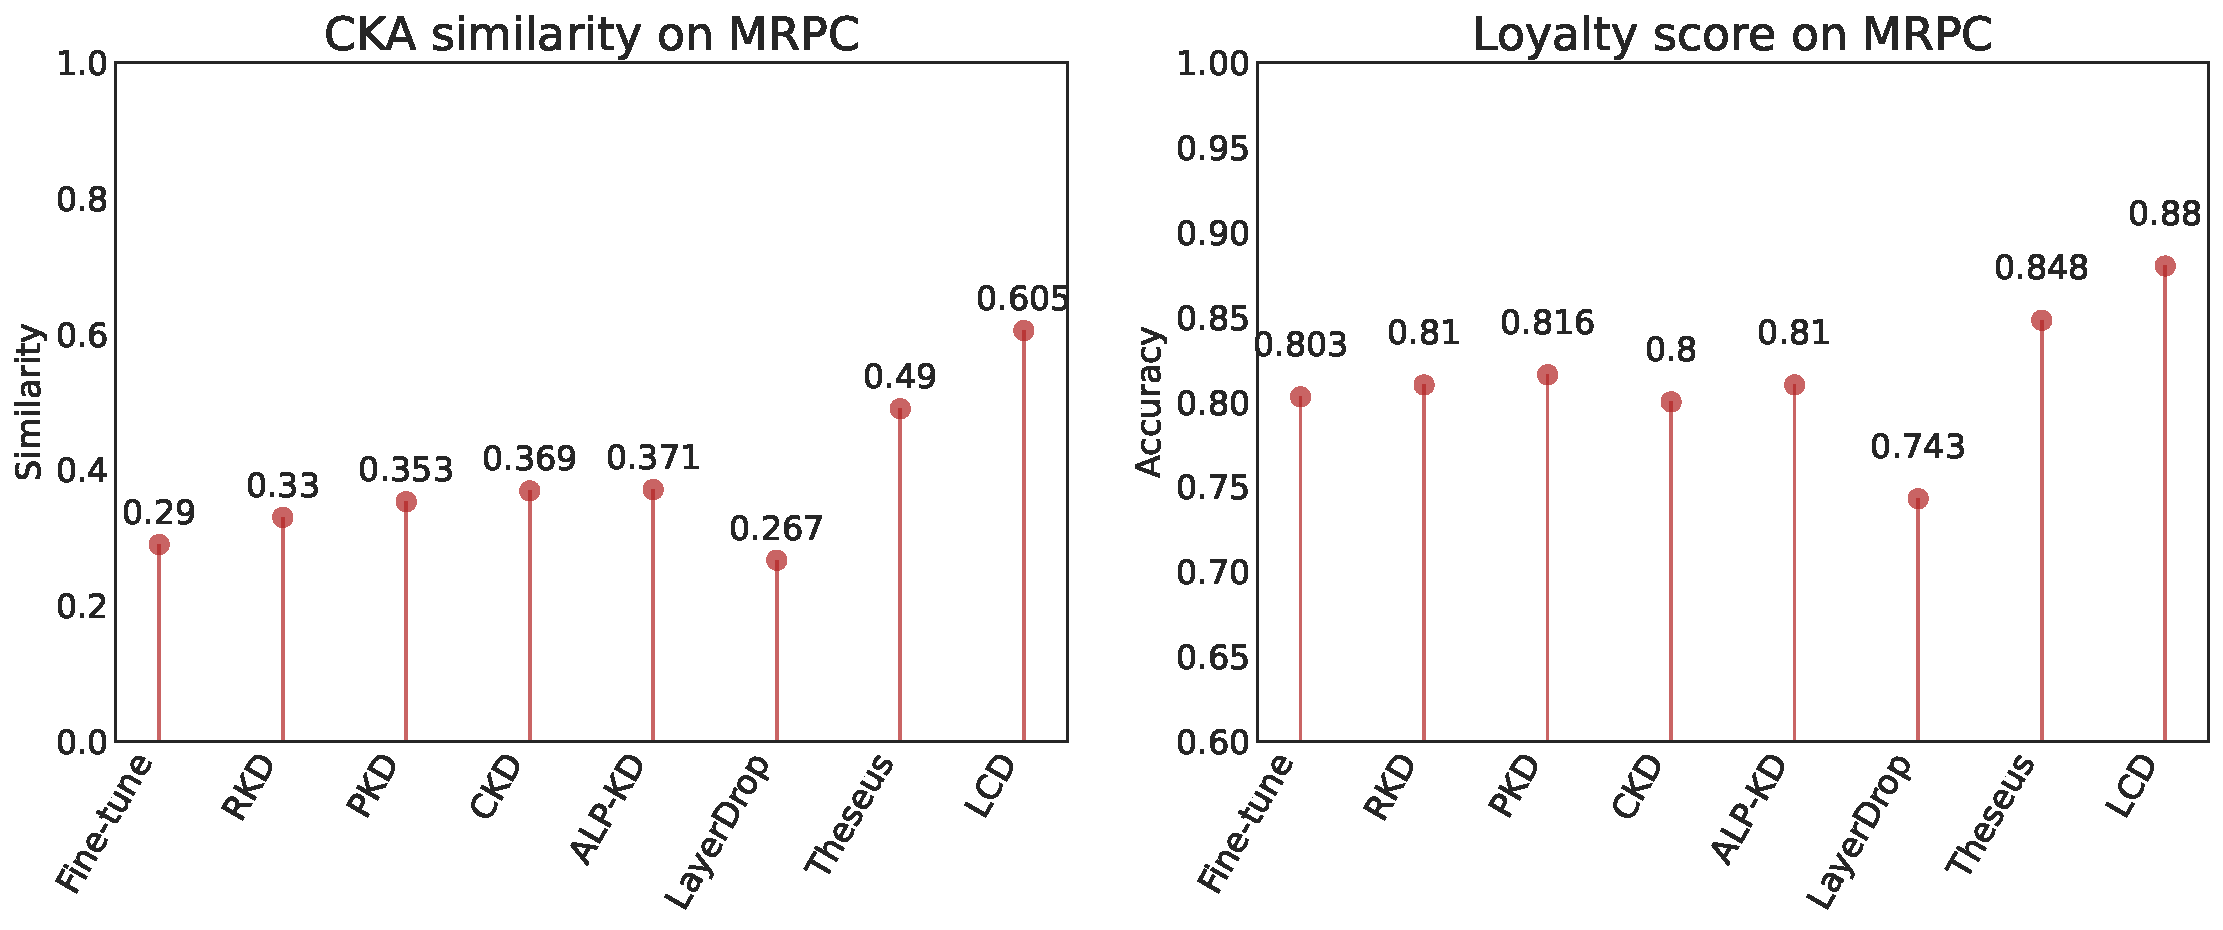
\includegraphics{./figures/cka_mrpc_all.pdf}}
    \caption{Loyalty and CKA similarity w.r.t. teacher network.}
    \label{fig:analysis_2}
\end{figure}

To examine the extent to which a complete student network mimics its teacher network, we focus on two aspects: prediction similarity and representation similarity. 
For prediction similarity, we calculate each student's accuracy by using teacher's prediction as ground-truth, which is referred to as loyalty score in \cite{byd} . For representation similarity, we employ the linear kernel CKA to calculate the similarity between the hidden states of CLS token.


The results are shown in \figref{fig:analysis_2}. The prediction similarity and representation similarity of student networks compressed by each method corresponding to the teacher network exhibit a positive correlation. Among all compared methods, LCD shows the highest degree of alignment with the teacher network in terms of both predictive and representational behavior, hence being the most promising to 
compress more powerful teacher network. Due to the space limit, please refer to the Appendix for the analyses of other datasets.
